%%%%%%%%%%%%%%
%% PREAMBLE %%
%%%%%%%%%%%%%%
\documentclass[10pt,twoside,twocolumn,openany,nomultitoc]{book}

%% PACKAGES %%
\usepackage[layout=true]{dnd}
\usepackage[english]{babel}
\usepackage[utf8]{inputenc}
\usepackage[singlelinecheck=false]{caption}
\usepackage{amssymb}
\usepackage{lipsum}
\usepackage{listings}
\usepackage{shortvrb}
\usepackage{stfloats}
\usepackage{csquotes}
\usepackage{textcomp}
\usepackage{xcolor}
\usepackage{graphicx}
\usepackage{titling}
\usepackage{verbatim}
\usepackage{setspace}
\usepackage{courier}
\usepackage[export]{adjustbox}
\usepackage{glossaries}
\usepackage[backend=biber,
        style=apa,        
        isbn=false,
        firstinits=true,
        ]{biblatex}

%% CONFIG %%
\captionsetup[table]{labelformat=empty,font={sf,sc,bf,},skip=0pt}
\MakeShortVerb{|}
\lstset{%
  basicstyle=\ttfamily,
  language=[LaTeX]{TeX},
  breaklines=true,
}

%% GENERATE APPENDIX %%
\addbibresource{bibliography.bib}
\makeglossaries

%%%%%%%%%%
% TITLE PAGE %
%%%%%%%%%%

 \title{Language \& Labyrinths\\{%
    %
\includegraphics[width=\textwidth]{img/buildingmen.png}} \\
\large A Metalinguistic Journey through Erdogic Literature}}
\author{Multiplex Void}
\date{2022/04/25}

%%%%%%%%%%%%%%%%%%%%
%%      BEGIN DOCUMENT      %%
%%%%%%%%%%%%%%%%%%%%
\begin{document}

\thispagestyle{empty}
 \begin{tikzpicture}[remember picture,overlay]
   \node at (current page.center) {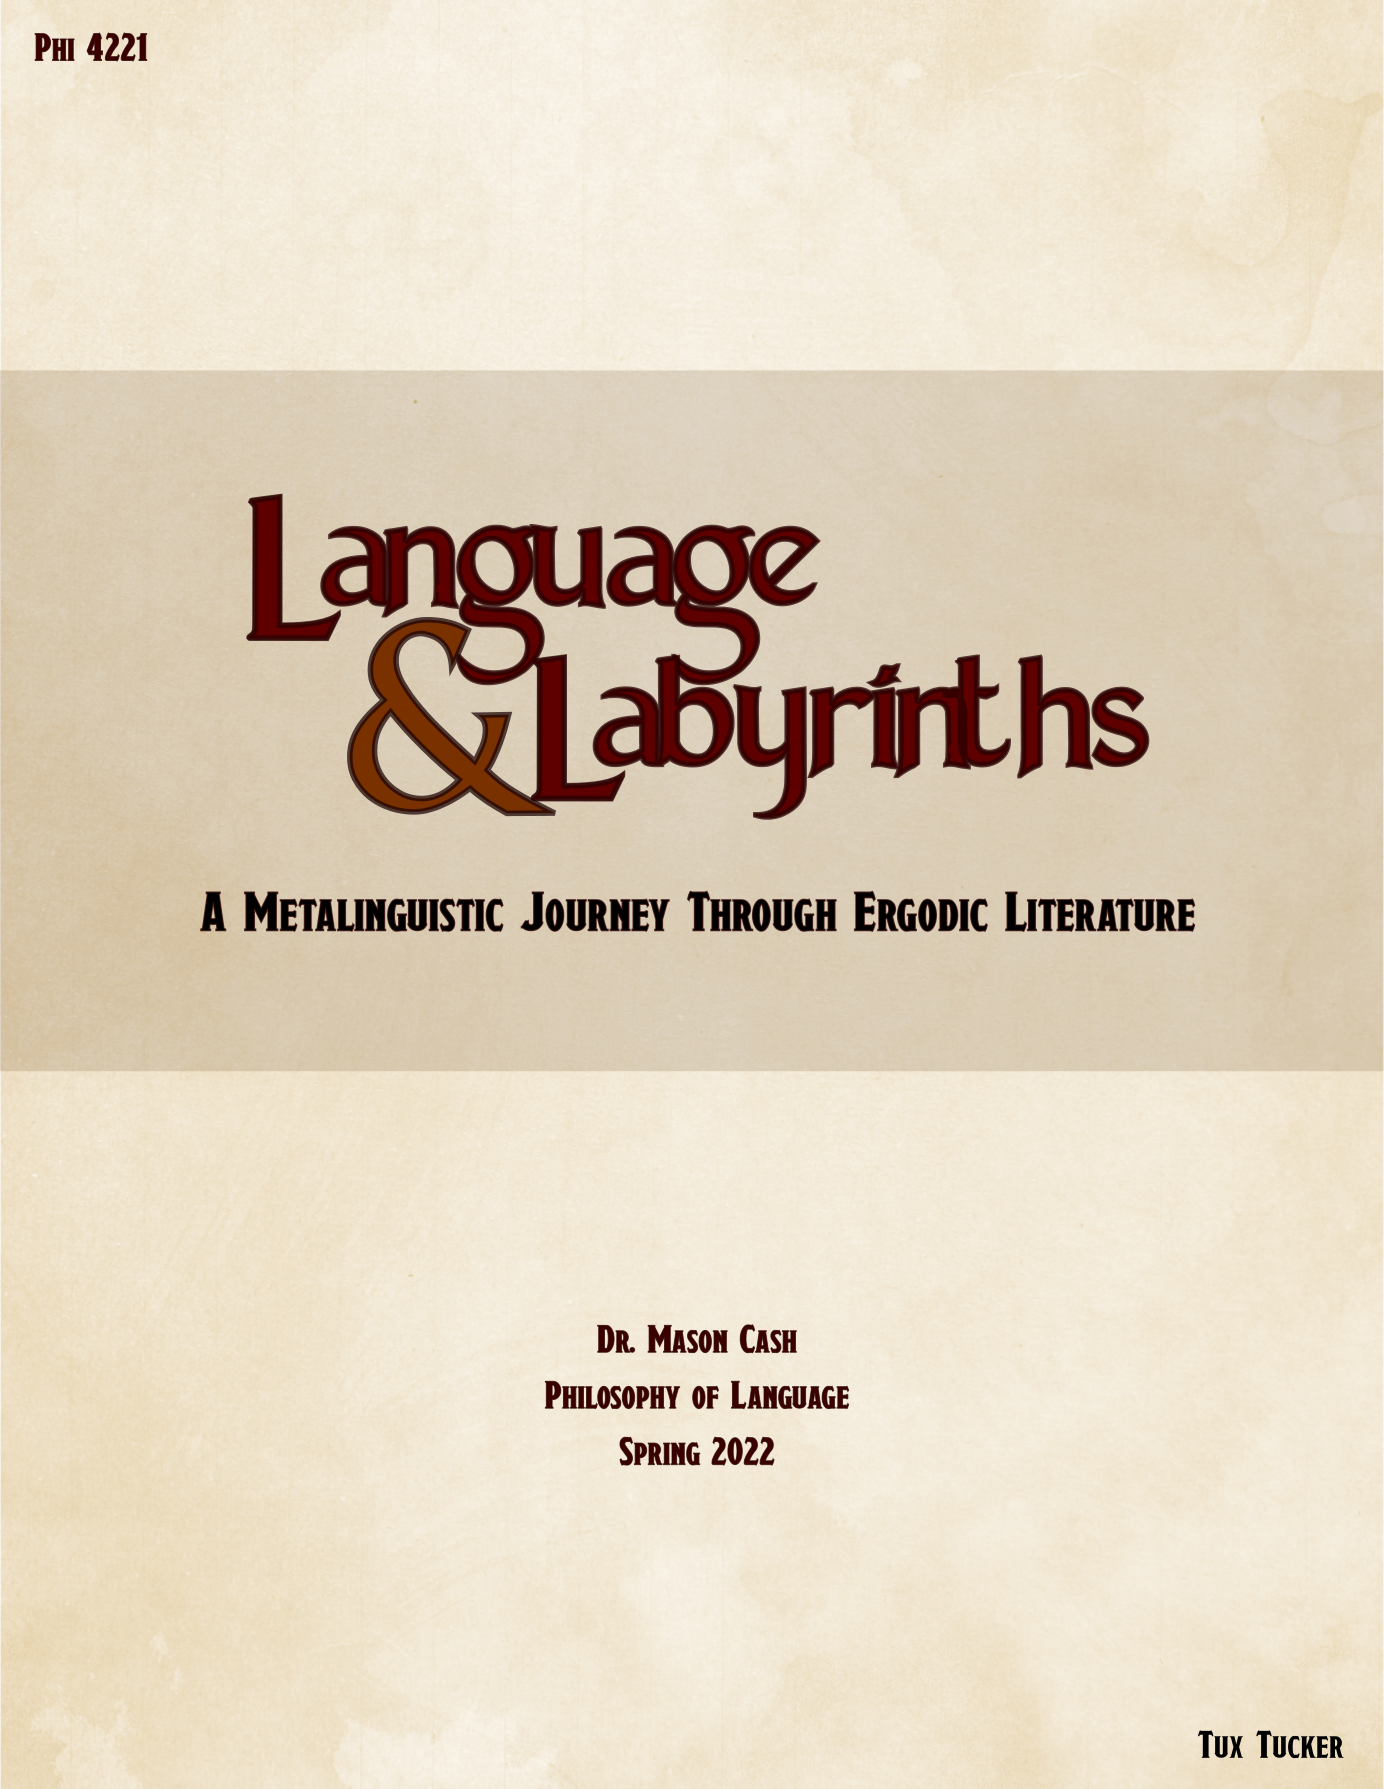
\includegraphics[width=\pdfpagewidth,height=\pdfpageheight]{img/LnL-title-page.png}};
 \end{tikzpicture}

\tableofcontents
\mainmatter

%%%%%%%%%%%%%%%%%%%%%%%%%%
%%	CHAPTER		%%
%%    INTRODUCTION	%%
%%%%%%%%%%%%%%%%%%%%%%%%%%
\part{Introduction}   %%

%%%%%%%%%%%%%%%%%%%%%%%
%%% ABOUT THIS WORK %%%
\chapter{About this Work}

\DndDropCapLine{I}{t seems only appropriate to present } a paper on ergodic literature in ergodic format--in fact, I would argue that such an approach is necessary to properly convey the ideas and concepts contained within this tome. By its very nature, ergodic literature demands active engagement on the part of its 
|Reader(s)|.%
    \footnote{The term |Reader| is perhaps too restrictive in describing the role of one who engages with literature of this form. It may be more accurate to consider this individual a |user| or |consumer| of ergodic media. Moreover, such  an individual need not act alone. Many ergodic works, such as MUDs, ARGs, and tabletop RPGs, require the participation and cooperation of multiple individuals for storytelling and puzzle-solving purposes.}         
It requires not only \textit{interpretation} but \textit{reciprocation}. It is not meant to be \textit{consumed}, but \textit{explored}. Only through non-trivial effort can one effectively traverse such work. \\ 

In this introductory section and following chapters, I will define ergodic literature, explain its origins, present contemporary examples, and describe the advantages of ergodic media over more traditional means in engaging the reader on an interactive level. Furthermore, I will take time to explain my own intentions as author, and justify the means through which I have chosen to communicate these concepts.
%e.g., by including them as a canonical part of the text. 

%% SIDEBAR: HISTORY OF TERMS %%
\begin{DndSidebar}[]{History of Terms}
    The term |Ergotic Literature| was first defined by Espen J. Aarceth in his 1997 book \textit{Cybertext}. It is derived from the Greek |ergon| and |hodos|, meaning \textit{work} and \textit{path}, respectively. The term |Cybertext| was first defined in Norbert Wiener's 1948 book \textit{Cybernetics}. It is derived from the Greek |kybernetes|, meaning \textit{steersman}.
\end{DndSidebar}
    
%%%%%%%%%%%%%%%%%%%%%%%%%%%
%% DUNGEONS AND DIALOGUE %%
\subsection{Dungeons and Dialogue}
\DndDropCapLine{T}{his work is presented in the style } of a 5e Dungeons and Dragons manual. Why this format, and not another? As the Author of this text, I knew from the beginning that I was going to take an ergodic approach to this assignment. Initially, I had planned on taking on a form inspired by \texttt{\color{blue}House} \color{black} of Leaves. It is a favorite of mine, after all, and has shaped a great deal of my own thoughts and perspectives. However, implementing this proved difficult:  \texttt{\color{blue}House} \color{black}of Leaves is maddening-- intentionally so.  Immersing myself in the text never fails to induce in me an altered state of consciousness--we find ourselves consumed by a kind of madness. This mental state, while phenomenologically interesting, presents significant writing challenges. The thoughts are \textit{too} disorganized, too flighty and entangled and chaotic and confused. I was entirely unable to write in such a way that could properly translate these states and ideas from Author to Reader. Any level of understanding would require significant effort on the part of the Reader. \\\vspace{2pt}

That's asking a bit too much, I think. \\\vspace{2pt}

Beyond that, there were typesetting concerns-- trying to program all of this in \LaTeX\hspace{1pt}  was simply taking up too much of my time. Searching for an alternative approach, I eventually stumbled upon a DnD 5e  \LaTeX\hspace{1pt}  template--perfect! For one, a DnD manual is a perfect representation of ergodic text. It is not intended to be read like a novel (or a paper), from cover-to-cover in a linear fashion. Its format makes it perfectly suitable as a reference guide. This seemed particularly appropriate for this assignment.  What better way to explain and demonstrate ergodicity than by using this format to explore course themes and answer questions of interest?  Furthermore, I know that the primary Reader for whom this is intended is already quite familiar with tabletop guides, and thus there is a common context upon which to base this work. This means less explanation on my part and less confusion on theirs--a boon for all!\\
     
 %%%%%%%%%%%%%%%%%%%%%%%    
 %% READERS AND ROLES %%
 \subsection{Readers and Roles}   
    \DndDropCapLine{T}{he role that the Reader plays will} shape how they traverse this document.  Are they a (potential) |Player|? A |GM|? Perhaps they're curious about tabletop gaming, or perhaps they are unfamiliar with it entirely. Perhaps the Reader is myself, the |Author|, as I read and reread and organize and edit this document.

One particular Reader--our target audience--will play the role of \textit{'professor who is grading a student's assignment according to a specific rubric'.}%
        \footnote{Hello Dr. Cash!} 
More specifically, this Reader is known to be \textit{'a professor who is grading a student's assignment according to a specific rubric who already has familiarity with tabletop RPGs'} and thus, as previously mentioned, already shares a common cultural background with the author/student.

This gives us the advantage of being able to use tropes and jargon that the Reader is already familiar with and greatly simplifies the effort to communicate effectively. As I, the |Author|, will be playing the role of the |Student|, it would behoove us to detail how this document intends to fulfull the rubric assigned by the |Professor|. 
 
 %%%%%%%%%%%%%%%%%%%%%%
 %% REGARDING RUBRIC %%   
 \section{Regarding Rubric}\vspace{6pt}
    \DndDropCapLine{I}{will now explain how this document } follows the guidelines defined in the course syllabus and how each section is intended to be interpreted. 
    
The |Research Paper|, accounting for 20-25\% of the total course grade, is to contain \textasciitilde 3000 words and include substantial discussion of at least two course readings and two academic works, with citations. |Part 1| and its chapters are intended to fulfil these criteria. %% fix tildes
    
The |Short Paper|, accounting for 15\% of the total course grade, is to contain \textasciitilde 1000 words while answering a question or taking a position on a specific topic of interest that aligns with course themes. Requirements for the |Final Reflections| are similar. These assignments are contained in |Part II: Sessions|, which takes form of dialogue between philosophers whose works have been covered in class. Taking the role of DnD players, they will discuss and debate topics of linguistic interest. 
    
For those experienced in tabletop roleplaying, the style and content of these arguments may be familiar. Who among us hasn't gotten into a squabble over interpretation over the particulars of rules? Who hasn't engaged in hearty debate over RAW vs. RAI only to be shot down by ROG? These Sessions are designed to be thoughtful, but playful. 

%%%%%%%%%%%%%%%%%%%%%%%
%% BEYOND THE BASICS %%
%\vfill\null  
 \vspace{10pt} 
 \section{Beyond the Basics}\vspace{2pt}
 \DndDropCapLine{A}{great deal of effort has been } expended in order to keep the formatting of this document true to form. As an ergodic work, we consider the document's style, as well as the code written to produce it, as essential as the text itself. Therefore, in order to more fully comprehend this project as a whole, we heartily encourage the Reader to explore the \textit{Language and Labyrinths} |github|%
    \footnote{https://github.com/agoramachina/\\\hspace{6pt}Language-and-Labyrinths.git} repository. \\

The |git| commit log itself is a record of how this paper evolved over time.  Particular note should be taken of the files |Language & Labyrinths.tex|, |bibliography.bib|, and |glossary.tex|. These documents form the core of our work: the |.tex| file is compiled with the |.bib| bibliography and |.tex| glossary by \LaTeX\vspace{1pt} to produce the final |.pdf|. Great care has been taken to ensure that the code is well-organized and heavily documented so that even a viewer with minimal programming experience can understand how this work was created. \\\vspace{12pt}

Images for the Title Page were generated with |gnofract4d|. These images and the code to produce them are included in the |img| directory. 

This work and all content is published under the open source |MIT License|. The libraries used for our template are based on the |DnD-5e-LaTeX-Template|%
    \footnote{https://github.com/rpgtex/DND-5e-LaTeX-Template.git} published by |rpgtex|. 

 Neale Davidson is the author of the |Draconis| font used in the cover text.   
     \vspace{4pt} 
     
For further instruction, consult the project's README.      
    
%%%%%%%%%%%%%%%%%%%%%%%%%%
%%	CHAPTER 2	%%
%% EXPLORING ERGODICITY %%
%%%%%%%%%%%%%%%%%%%%%%%%%%
\chapter{Exploring Erdogicity} 
\section{A Lesson in Language}\vspace{2pt}
     \DndDropCapLine{W}{hat is the purpose of language?} What is it \textit{for}?
     And what exactly \textit{is} language, anyway? These questions form the necessary foundation for further linguistic inquiry: What forms can language take? What is the language of story, of narrative, of literature? Of games and play? What can we possibly say about language, and what can language possibly say about us?

%% Discussing Discourse %%     
\subsection{Discussing Discourse}

\DndDropCapLine{B}{efore we can begin to answer these} questions, the complication of circularity greets us at the outset: in order to discuss language, we must \textit{use} language. Whether this is taken as an insurmountable challenge or not depends on one's approach.
     
Those following the \textit{Analytic} tradition of philosophy have typically emphasized the formal characteristics of language. Linguists of this variety tend to prioritize abstraction over synthesis, paying particular attention to a statement's grammar and syntax \parencite{putnam1962analytic}.%
    \footnote{This is perhaps unsurprising, given that the language of logic and mathematics is established a common underpinning of analytical linguistics. A search to apply such rigor to natural language is a common goal of such approaches.}
For the analytic philosopher, the primary purpose of language is to express truth statements.  \\
    \vspace{2pt}

%% ANALYTIC PHILOSOPHY
\subsubsection{Analytic Philosophers' Guild}
%% WITTGENSTEIN
    \begin{DndComment}{Ludwig Wittgenstein (1889-1951)}
    In his \textit{Tractatus Logico-Philosophicus} and \textit{Philosophical Investigations}, Ludwig Wittgenstein attempts to develop a comprehensive model of language--an ideal, nonambiguous language of philosophical inquiry--on the foundation of structural characteristics and correlations of language.  Though a lofty endeavor, Wittgenstein himself notes in his \textit{Philosophical Investigations} that this task would remain incomplete (vi). 
    \end{DndComment} 
%% FREGE
    \begin{DndComment}{Gottlob Frege (1848-1925)}
    Frege's conceptual notation of language sought to address the problems of ambiguity and fludity in natural language \parencite[p. 4]{big-questions}.
    \end{DndComment}
%% QUINE
    \begin{DndComment}{W.V. Quine (1908-2000)}
    lorem
    \end{DndComment}
%% DAVIDSON    
    \begin{DndComment}{Donald Davidson (1917-2003)}
    ipsum
    \end{DndComment}
    
        
In contrast, those of the \textit{Continental} school of philosophy are oriented around    
beliefs, culture, perception; intention  
    
%% CONTINENTAL PHILOSOPHY
%% world disclosing; how language shapes experience
\subsubsection{Continental Philosophers' Guild}
%% BENVENISTE
    \begin{DndComment}{Émile Benveniste (1902-1976)}
   dolor
    \end{DndComment}     
%% HEIDEGGER
    \begin{DndComment}{Martin Heidegger (1889-1976)}
   dolor
    \end{DndComment}   

But what is form without content? How does the inner relate to the outer? 
Devoid of context

language is a living, dynamic thing. culturally bound
    

\section{Nature of Narrative}\vspace{2pt}

\section{Self as Subject}

\section{Transcending Text}
\subsection{Persons and Programs}

\section{Mapping the Meta}
  
\subsection{Form and Function}

%%%%%%%%%%
%% PART II %%    
%%%%%%%%%%%
%% SESSIONS %%
\part{Sessions}

%% SESSION 0 %%
\chapter{Session Zero}\vspace{6pt}

\begin{DndReadAloud}
  \lipsum[1]
\end{DndReadAloud}

%% 

\section{On Language}

\section{On Translation}
    \lipsum[1]
\section{On Knowing}
    \lipsum[2]
\section{On Reference}
    \lipsum[3]
    
%% ERRATA %%
\part{Errata}
%% DnD Reference %%
\chapter{Reference Material}

%%%%%%%%%
%% SPELLS %%
%%%%%%%%%%
\section{Spells}\vspace{6pt}

%% SENDING %%
    \DndSpellHeader%
      {Sending}
      {3rd-level Evocation}
      {1 action}
      {Unlimited}
      {V, S, M (a short piece of fine copper wire)}
      {1 Round}
            You send a short message of twenty-five words or less to a creature with which you are familiar. The creature hears the message in its mind, recognizes you as the sender if it knows you, and can answer in a like manner immediately. The spell enables creatures with Intelligence scores of at least 1 to understand the meaning of your message. \\
            You can send the message across any distance and even to other planes of existence, but if the target is on a different plane than you, there is a 5 percent chance that the message doesn't arrive.
        
%% COMPREHEND LANGUAGES    %% 
    \DndSpellHeader%
      {Comprehend Languages}
      {1st Level Divination (Ritual)}
      {1 action}
      {Self}
      {V, S, M (a pinch of soot and salt)}
      {1 Hour}
    For the duration, you understand the literal meaning of any spoken language that you hear. You also understand any written language that you see, but you must be touching the surface on which the words are written. It takes about 1 minute to read one page of text. \\
    This spell doesn’t decode secret messages in a text or a glyph, such as an arcane sigil, that isn’t part of a written language.        
    
%% TONGUES %%    
    \DndSpellHeader%
      {Tongues}
      {3rd Level Divination}
      {Touch}
      {The creature you touch}
      {V, M (a small clay model of a ziggurat)}
      {1 Hour}
    This spell grants the creature you touch the ability to understand any spoken language it hears. Moreover, when the target speaks, any creature that knows at least one language and can hear the target understands what it says.

            
%% CLASSES %%
\section{Classes}

\chapter{Appendix}
\section{Glossary}
\printglossaries

%% BIBLIOGRAPHY %%

\section{Bibliography}
\begingroup
\let\clearpage\relax

    \nocite{*}

    \onecolumn{
        \setstretch{1.5}
        \printbibliography[heading=none]}
    \endgroup




%----------------------------------------------------------------------------------------
%	BIBLIOGRAPHY
%----------------------------------------------------------------------------------------



\end{document}
